\documentclass[pdftex,12pt,a4paper]{report}

\usepackage[portuguese,english]{babel}
\usepackage[T1]{fontenc} 
\usepackage[table]{xcolor}
\usepackage[utf8]{inputenc}
\usepackage[pdftex]{graphicx}
\usepackage{minitoc}
\usepackage{hyperref}
\usepackage{indentfirst}
\usepackage[compact]{titlesec}
\usepackage{fancyhdr}
\usepackage{caption}
\usepackage{pgfplots}
\usepackage{pgfplotstable}
\usepackage{fixltx2e}
\usepackage{mathtools}
\usepackage{fancyhdr}
\usepackage{listings}
\usepackage{color}
\usepackage{sverb}
\usepackage[section]{placeins}
%Highlight
\newcommand{\shellcmd}[1]{\\\indent\indent\texttt{\footnotesize\# #1}\\}

\pagestyle{fancy}
\renewcommand*\thesection{\thechapter\arabic{section}}
\newcommand{\HRule}{\rule{\linewidth}{0.5mm}}
\begin{document}

\begin{titlepage}

\begin{center}


\includegraphics[width=0.15\textwidth]{./logo}\\[0.5cm]    

\textsc{\large Universidade de Aveiro \\[1cm]\large departamento de electrónica, telecomunicações e informática}\\[1cm]

\textsc{\large{47022}\large - Arquitectura de Computadores Avançada \\[1cm]}

\HRule \\[0.5cm]
{ \huge \bfseries  Home group assignment 1}\\[0.4cm]
{ \large \bfseries Implementing a forwarding and stall unit in a pipelined architecture}\\[0.4cm]
\HRule \\[1cm]

\textsc{\small{8240 - MESTRADO INTEGRADO EM ENGENHARIA DE COMPUTADORES E TELEMÁTICA}}\\[1cm]

\begin{minipage}{0.4\textwidth}

\begin{flushleft} \large
\href{mailto:rafael.ferreira@ua.pt}{António Rafael da \\ Costa Ferreira }
 \small{\\NMec: 67405 | P4G1}
\end{flushleft}
\end{minipage}
\begin{minipage}{0.4\textwidth}

\begin{flushright} \large
\href{mailto:rodrigocunha@ua.pt}{Rodrigo Lopes \\ da Cunha}
\small{\\NMec: 67800 | P4G1}
\end{flushright}
\end{minipage}\\[1cm]

{\large Docentes: Nuno Lau/José Luís Azevedo   }\\[0.5cm]

\vfill

{\large Novembro de 2015 \\ 2015-2016}

\end{center}

\end{titlepage} %Titulo do Relatorio
\renewcommand{\headrulewidth}{0pt}

%Cabeçalhos de rodapé
\fancyhead{}
\fancyfoot{}
\lhead{Home group assignment 1}
\rhead{ACA - 2015/2016}
\lfoot{Rafael Ferreira nmec: 67405 \\ Rodrigo Cunha nmec: 67800}
\rfoot{\thepage}

%Renomear Comandos
\renewcommand*\contentsname{Conteúdos}
\renewcommand*\figurename{Figura}
\renewcommand*\tablename{Tabela}

%Conteúdos, dar paragrafo
\tableofcontents
%Headers
\renewcommand{\headrulewidth}{0.15pt}
\renewcommand{\thechapter}{}

\clearpage

\section{Introdução}
% o que, porquê e o objetivo

O trabalho proposto para a unidade curricular de Arquitetura de Computadores Avançada é a implementação de uma nova fase pipeline que resulta da divisão da fase já existente ID, ficando assim duas fases ID1 e ID2.

A primeira entrega é constituída pela implementação desta nova fase, sem forwarding, e é apenas pedido que sejam introduzidos os stalls e que as operações de salto condicional e incondicional sejam resolvidas nesta nova fase.

Já a segunda entrega consiste na evolução da pipeline através da introdução de forwarding, que reduz significativamente alguns stall. Não sendo possível através de forwarding remover todos os stalls, foi então pedido também que se introduzissem apenas os stalls necessários nesta actualização da pipeline.

O relatório reflete uma descrição das condições introduzidas tanto para forwarding como hazards, assim como testes e exemplos para demonstração destas condições e exercícios propostos, e por último a conclusão deste mesmo trabalho.

\newpage
\section{Exercício 1}

\subsection{Divisão da fase ID em duas fases ID1/ID2}
Neste primeiro exercício, era pedido que se fizesse a divisão da fase ID, por duas fases ID1 e ID2.

\begin{figure}[!htb]
\center
 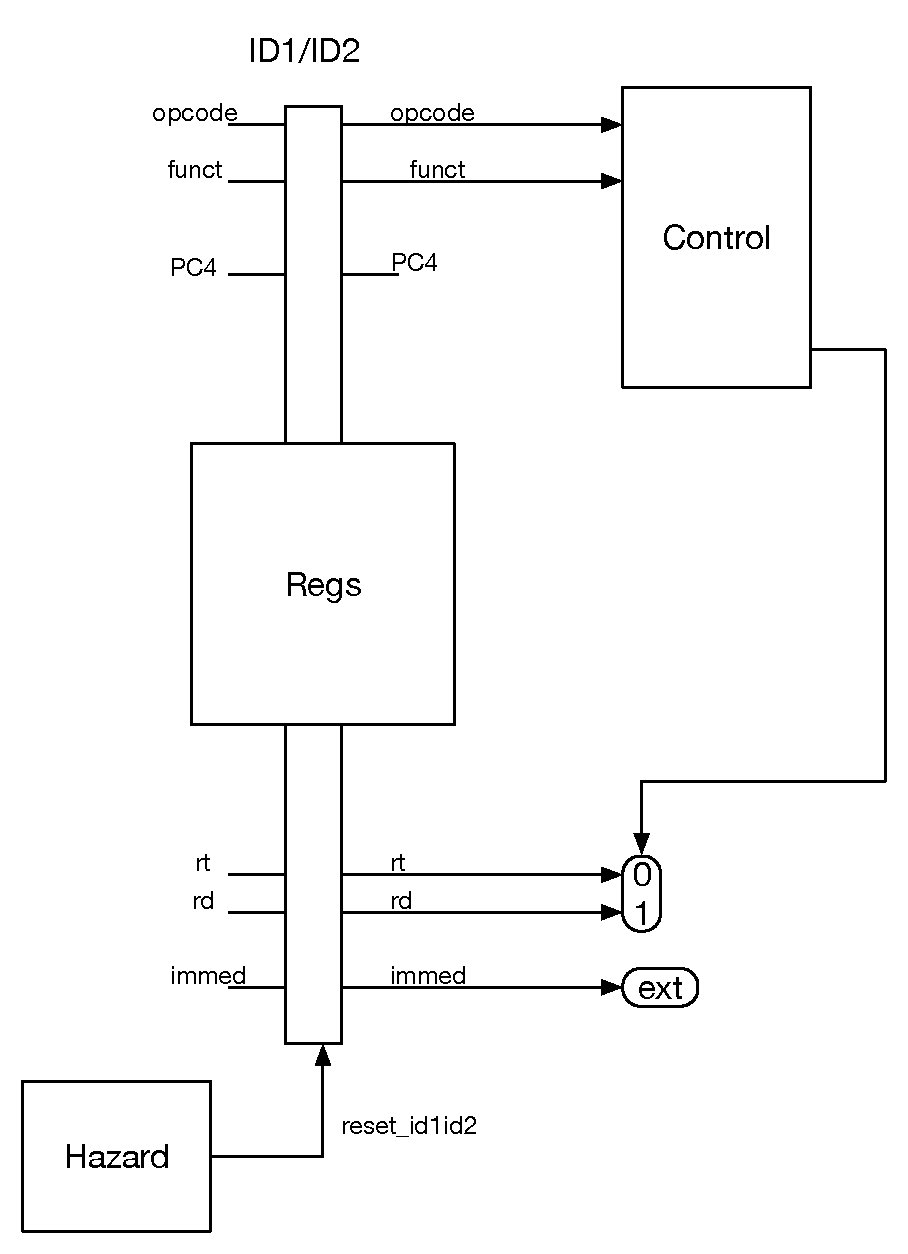
\includegraphics[width=100mm,scale=1]{ID1ID2ex1.pdf}
 \caption{\\ Registo ID1/ID2}
 \label{fig:ex1RegID1ID2}
\end{figure}

O inicio da leitura de registos tem inicio em ID1 e termina em ID2 (como podemos verificar na figura 1), sendo que na fase ID1 também é feito o decode da instrução para obter os sinais de rs, rt, rd, funct, opcode e immed.  Tudo o que se resolvia em ID agora resolve-se em ID2, como por exemplo a unidade de Controlo, o extend e o Mux entre o rt e o rd.

Para este primeiro exercício criou-se um novo barramento de registos ID1/ID2, que toma como entradas o \textit{opcode}, o \textit{funct}, o \textit{immed}, o \textit{rt}, o \textit{rs} e o \textit{rd} vindos do decoder de ID1, sendo as saídas as correspondentes a estas mesmas portas. Existe também uma entrada vinda da unidade de Hazard, \textit{reset\_id1id2}, para fazer reset a este registo aquando da necessidade de existirem stalls ou branchs.

Na unidade de hazard foram feitas algumas alterações para que estes fossem resolvidos em ID2, que anteriormente eram resolvidos em ID. A única diferença é que são os registos em ID2, rs e rt, que definem a existência de hazard tendo em conta as fases mais avançadas da pipeline, como EXE, MEM e WB.

As condições para a existência de hazards são:


\begin{lstlisting}[language=c]
rs_id2.read()!=0 && rs_id2.read()==WriteReg_exe.read() 
&& RegWrite_exe.read()==true 
|| rt_id2.read()!=0 && rt_id2.read()==WriteReg_exe.read() 
&& RegWrite_exe.read()==true && MemRead.read()== false
\end{lstlisting} 

\begin{table}[!htb]
\centering
\label{my-label}
\resizebox{\textwidth}{!}{\begin{tabular}{ll|l|l|l|l|l|llll}
\cline{2-7}
\multicolumn{1}{l|}{add \$3, \$2, \$1} & IF & ID1 & ID2 & EXE                         & MEM                         & WB                          &                          &                          &                          &                         \\ \cline{2-11} 
add \$4, \$3, \$1                      &    & IF  & ID1 & \cellcolor[HTML]{F8A102}ID2 & \cellcolor[HTML]{F8A102}ID2 & \cellcolor[HTML]{F8A102}ID2 & \multicolumn{1}{l|}{ID2} & \multicolumn{1}{l|}{EXE} & \multicolumn{1}{l|}{MEM} & \multicolumn{1}{l|}{WB} \\ \cline{3-11} 
\end{tabular}}
\end{table}

Nestas primeiras condições estudamos os casos em que o registo rs ou rt da instrução que está em ID2, é o registo onde vai ser escrito pela instrução que se encontra em EXE, pelo que é necessário a existência de stalls. 

\begin{lstlisting}[language=c]
rs_id2.read()!=0 && rs_id2.read()==WriteReg_mem.read() 
&& RegWrite_mem.read()==true
|| rt_id2.read()!=0 && rt_id2.read()==WriteReg_mem.read() 
&& RegWrite_mem.read()==true && MemRead.read() == false
\end{lstlisting}

\begin{table}[!htb]
\centering
\label{my-label}
\resizebox{\textwidth}{!}{\begin{tabular}{lll|l|l|l|l|llll}
\cline{2-7}
\multicolumn{1}{l|}{add \$3, \$2, \$1} & \multicolumn{1}{l|}{IF} & ID1 & ID2 & EXE & MEM                                                & WB                          &                          &                          &                          &                         \\ \cline{2-8}
add \$0, \$0, \$0                      & \multicolumn{1}{l|}{}   & IF  & ID1 & ID2 & EXE                                                & MEM                         & \multicolumn{1}{l|}{WB}  &                          &                          &                         \\ \cline{3-11} 
add \$4, \$3, \$1                      &                         &     & IF  & ID1 & \cellcolor[HTML]{F8A102}{\color[HTML]{000000} ID2} & \cellcolor[HTML]{F8A102}ID2 & \multicolumn{1}{l|}{ID2} & \multicolumn{1}{l|}{EXE} & \multicolumn{1}{l|}{MEM} & \multicolumn{1}{l|}{WB} \\ \cline{4-11} 
\end{tabular}}
\end{table}

Para os casos em que o registo rs ou rt da instrução que está em ID2, é o registo onde vai ser escrito pela instrução que se encontra em MEM, pelo que continua a existir a necessidade de stalls.

\begin{lstlisting}[language=c]
rs_id2.read()!=0 && rs_id2.read()==WriteReg_wb.read() 
&& RegWrite_wb.read() == true
|| rt_id2.read()!=0 && rt_id2.read()==WriteReg_wb.read() 
&& RegWrite_wb.read() == true && MemRead.read() == false
\end{lstlisting} 

\begin{table}[!htb]
\centering
\label{my-label}
\resizebox{\textwidth}{!}{\begin{tabular}{llll|l|l|l|llll}
\cline{2-7}
\multicolumn{1}{l|}{add \$3, \$2, \$1} & \multicolumn{1}{l|}{IF} & \multicolumn{1}{l|}{ID1} & ID2 & EXE & MEM & WB                          &                          &                          &                          &                         \\ \cline{2-8}
add \$0, \$0, \$0                      & \multicolumn{1}{l|}{}   & \multicolumn{1}{l|}{IF}  & ID1 & ID2 & EXE & MEM                         & \multicolumn{1}{l|}{WB}  &                          &                          &                         \\ \cline{3-9}
add \$0, \$0, \$0                      &                         & \multicolumn{1}{l|}{}    & IF  & ID1 & ID2 & EXE                         & \multicolumn{1}{l|}{MEM} & \multicolumn{1}{l|}{WB}  &                          &                         \\ \cline{4-11} 
add \$4, \$3, \$1                      &                         &                          &     & IF  & ID1 & \cellcolor[HTML]{F8A102}ID2 & \multicolumn{1}{l|}{ID2} & \multicolumn{1}{l|}{EXE} & \multicolumn{1}{l|}{MEM} & \multicolumn{1}{l|}{WB} \\ \cline{5-11} 
\end{tabular}}
\end{table}

Por último existem ainda os casos onde o registo rs ou rt que está em ID2, é o registo que vai ser escrito pela instrução que se encontra em WB, pelo que só no ciclo a seguir o valor estará disponível no banco de registos, obrigando a introdução de um stall.
\newpage
\section{Exercício 2}

Neste segundo exercício, foi-nos proposto para que todos os saltos condicionais e incondicionais, fossem resolvidos em ID2. Para isso foi criada uma unidade de branch, que através de entradas como \textit{opcode}, \textit{rsdata}, \textit{rtdata}, \textit{branch}, \textit{target}, \textit{imm\_ext} e \textit{PC4}, calcula o \textit{branchTaken}, que nos diz se existe salto ou não, e o \textit{branchTarget} (Figura 2).

\begin{figure}[!htb]
\center
 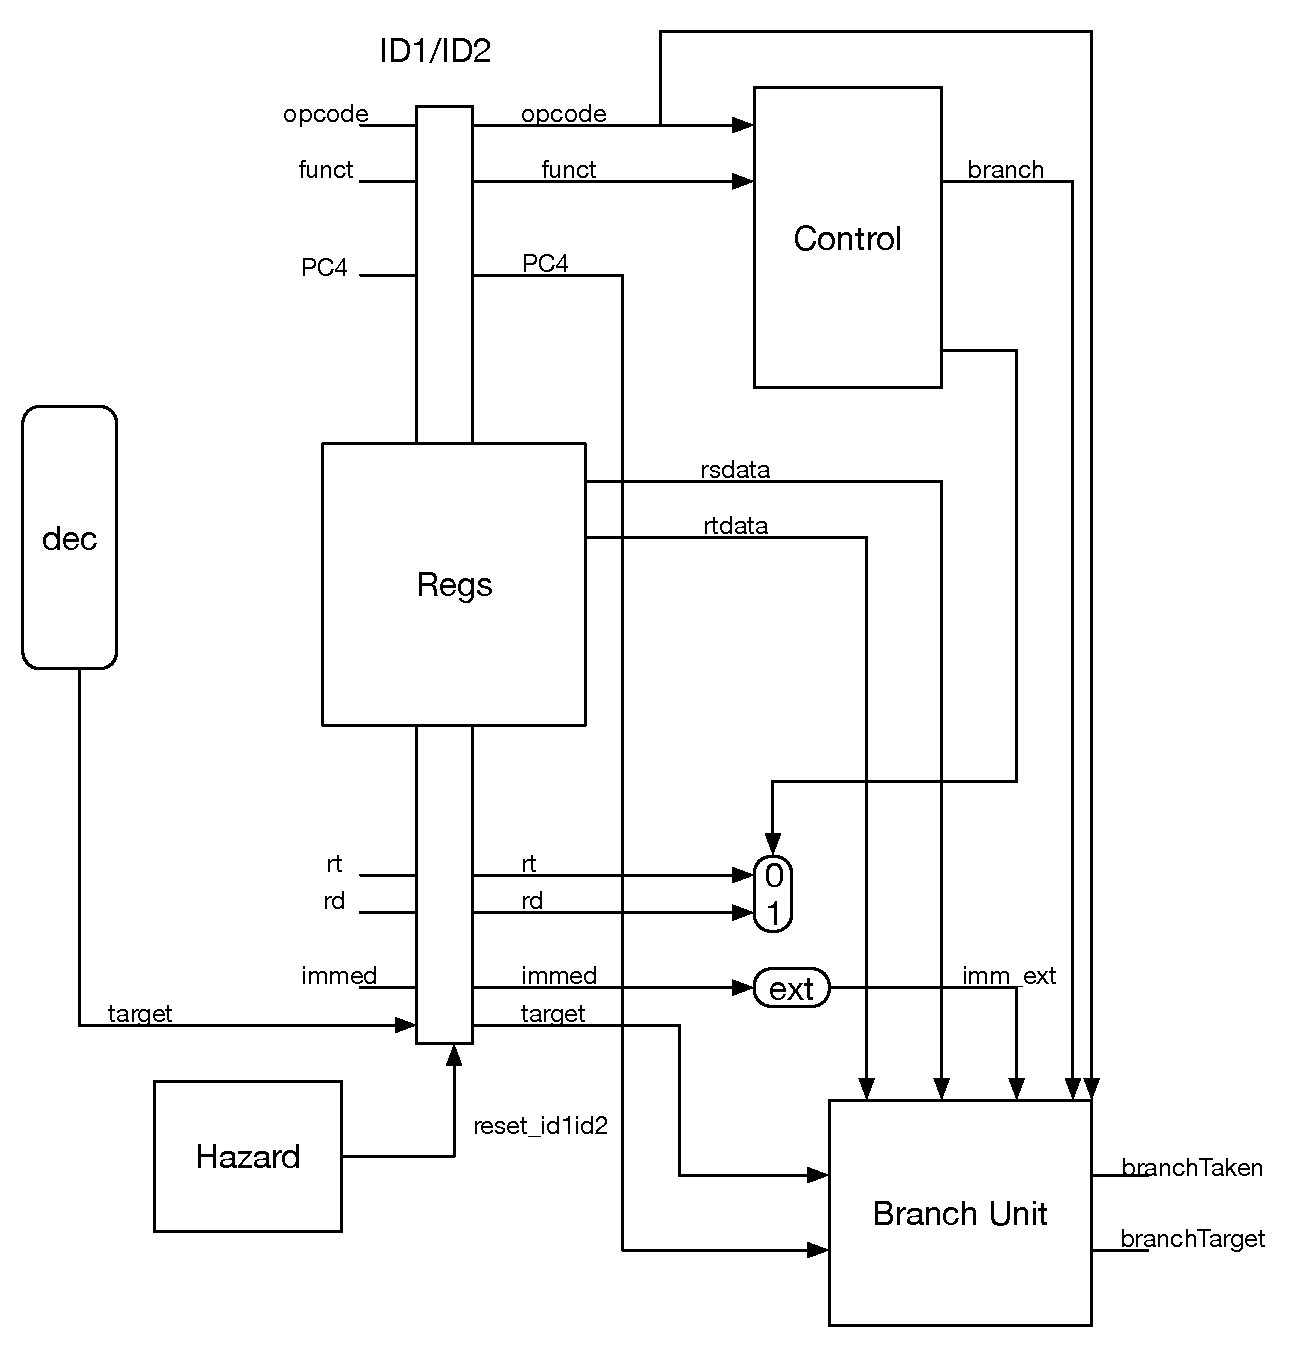
\includegraphics[width=100mm,scale=1]{ID1ID2ex2.pdf}
 \caption{\\Registo ID1ID2 com Branch Unit}\label{fig:ex2RegID1ID2}
\end{figure}

\subsection{Unidade de Branch}

Para que os saltos fossem resolvidos em ID2, foi necessário na unidade de branch resolver os mesmos. Para isto dentro da unidade de controlo, alterou-se a informação que a saída de branch possuí. Disponibilizaram-se mais bits para que esta saída indique na unidade de branch o tipo de salto que estamos a resolver.

Posto isto na unidade de branch, efetuam-se 6 casos diferentes:

\begin{itemize}
\item BEQ: compara se o valor de \textit{rsdata} é igual ao de \textit{rtdata}

\begin{lstlisting}[language=c]
if(rs.read() == rt.read()){
  branchTaken_res = true;
  branchTarget_res = PC4.read() + (imm_ext.read()<<2);
}else{
  branchTaken_res = false;
}
\end{lstlisting} 

\item BNE: compara se o valor de \textit{rsdata} é diferente de \textit{rtdata} 

\begin{lstlisting}[language=c]
if(rs.read() != rt.read()){
  branchTaken_res = true;
  branchTarget_res = PC4.read() + (imm_ext.read()<<2);
}else{
  branchTaken_res = false;
}
\end{lstlisting} 

\item BGTZ: compara se o valor de \textit{rsdata} é maior que zero

\begin{lstlisting}[language=c]
if((int)rs.read() > 0){
  branchTaken_res = true;
  branchTarget_res = PC4.read() + (imm_ext.read()<<2);
}else{
  branchTaken_res = false;
}
\end{lstlisting} 

\item BLEZ: compara se o valor de \textit{rsdata} é menor ou igual a zero

\begin{lstlisting}[language=c]
if((int)rs.read() <= 0){
  branchTaken_res = true;
  branchTarget_res = PC4.read() + (imm_ext.read()<<2);
}else{
  branchTaken_res = false;
}
\end{lstlisting} 

\item JUMP: salta para o target da instrução

\begin{lstlisting}[language=c]
branchTaken_res = true;
branchTarget_res = target32 << 2 | (PC4.read() & 0xF000);
\end{lstlisting} 

\item JR: salta para o valor de \textit{rsdata}

\begin{lstlisting}[language=c]
branchTaken_res = true;
branchTarget_res = rs.read();
\end{lstlisting} 

\end{itemize} 

Sendo os saltos resolvidos em ID2, foram removidos de fases mais avançadas unidades que não seriam mais utilizadas, como por exemplo o \textit{sl2} e a unidade de adição para branch em EXE e o \textit{and} em MEM. Os portos \textit{PC4} e \textit{branch} também deixaram de ser propagados para as fases seguintes à ID2.

\subsection{Unidade de Hazard adaptada para a nova resolução de saltos}

Para que instruções que entrem de forma errada na pipeline quando um branch ocorre sejam descartadas excepto a seguinte (delayed branch slot), foi necessário alterar na unidade de Hazard as fases às quais é necessário fazer reset. Desta feita quando a nossa unidade de Hazard trata de descartar instruções que entrem de forma errada na pipeline e de colocar stalls aquando da ocorrência destes.

\section{Forwarding}

Na tarefa 3 foi-nos pedido para identificar quais são os tipos de forwarding que podem ocorrer na nossa arquitetura onde a origem dos valores são os valores dos registos da pipeline e o seu destino é a "stage".

Os tipos de forwarding são:
\begin{itemize}
\item EXE/MEM->EXE
\item EXE/MEM->ID2
\item MEM/WB->EXE
\item MEM/WB->ID2
\item MEM/WB->MEM
\end{itemize} 

\newpage

\begin{figure}[!htb]
\center
 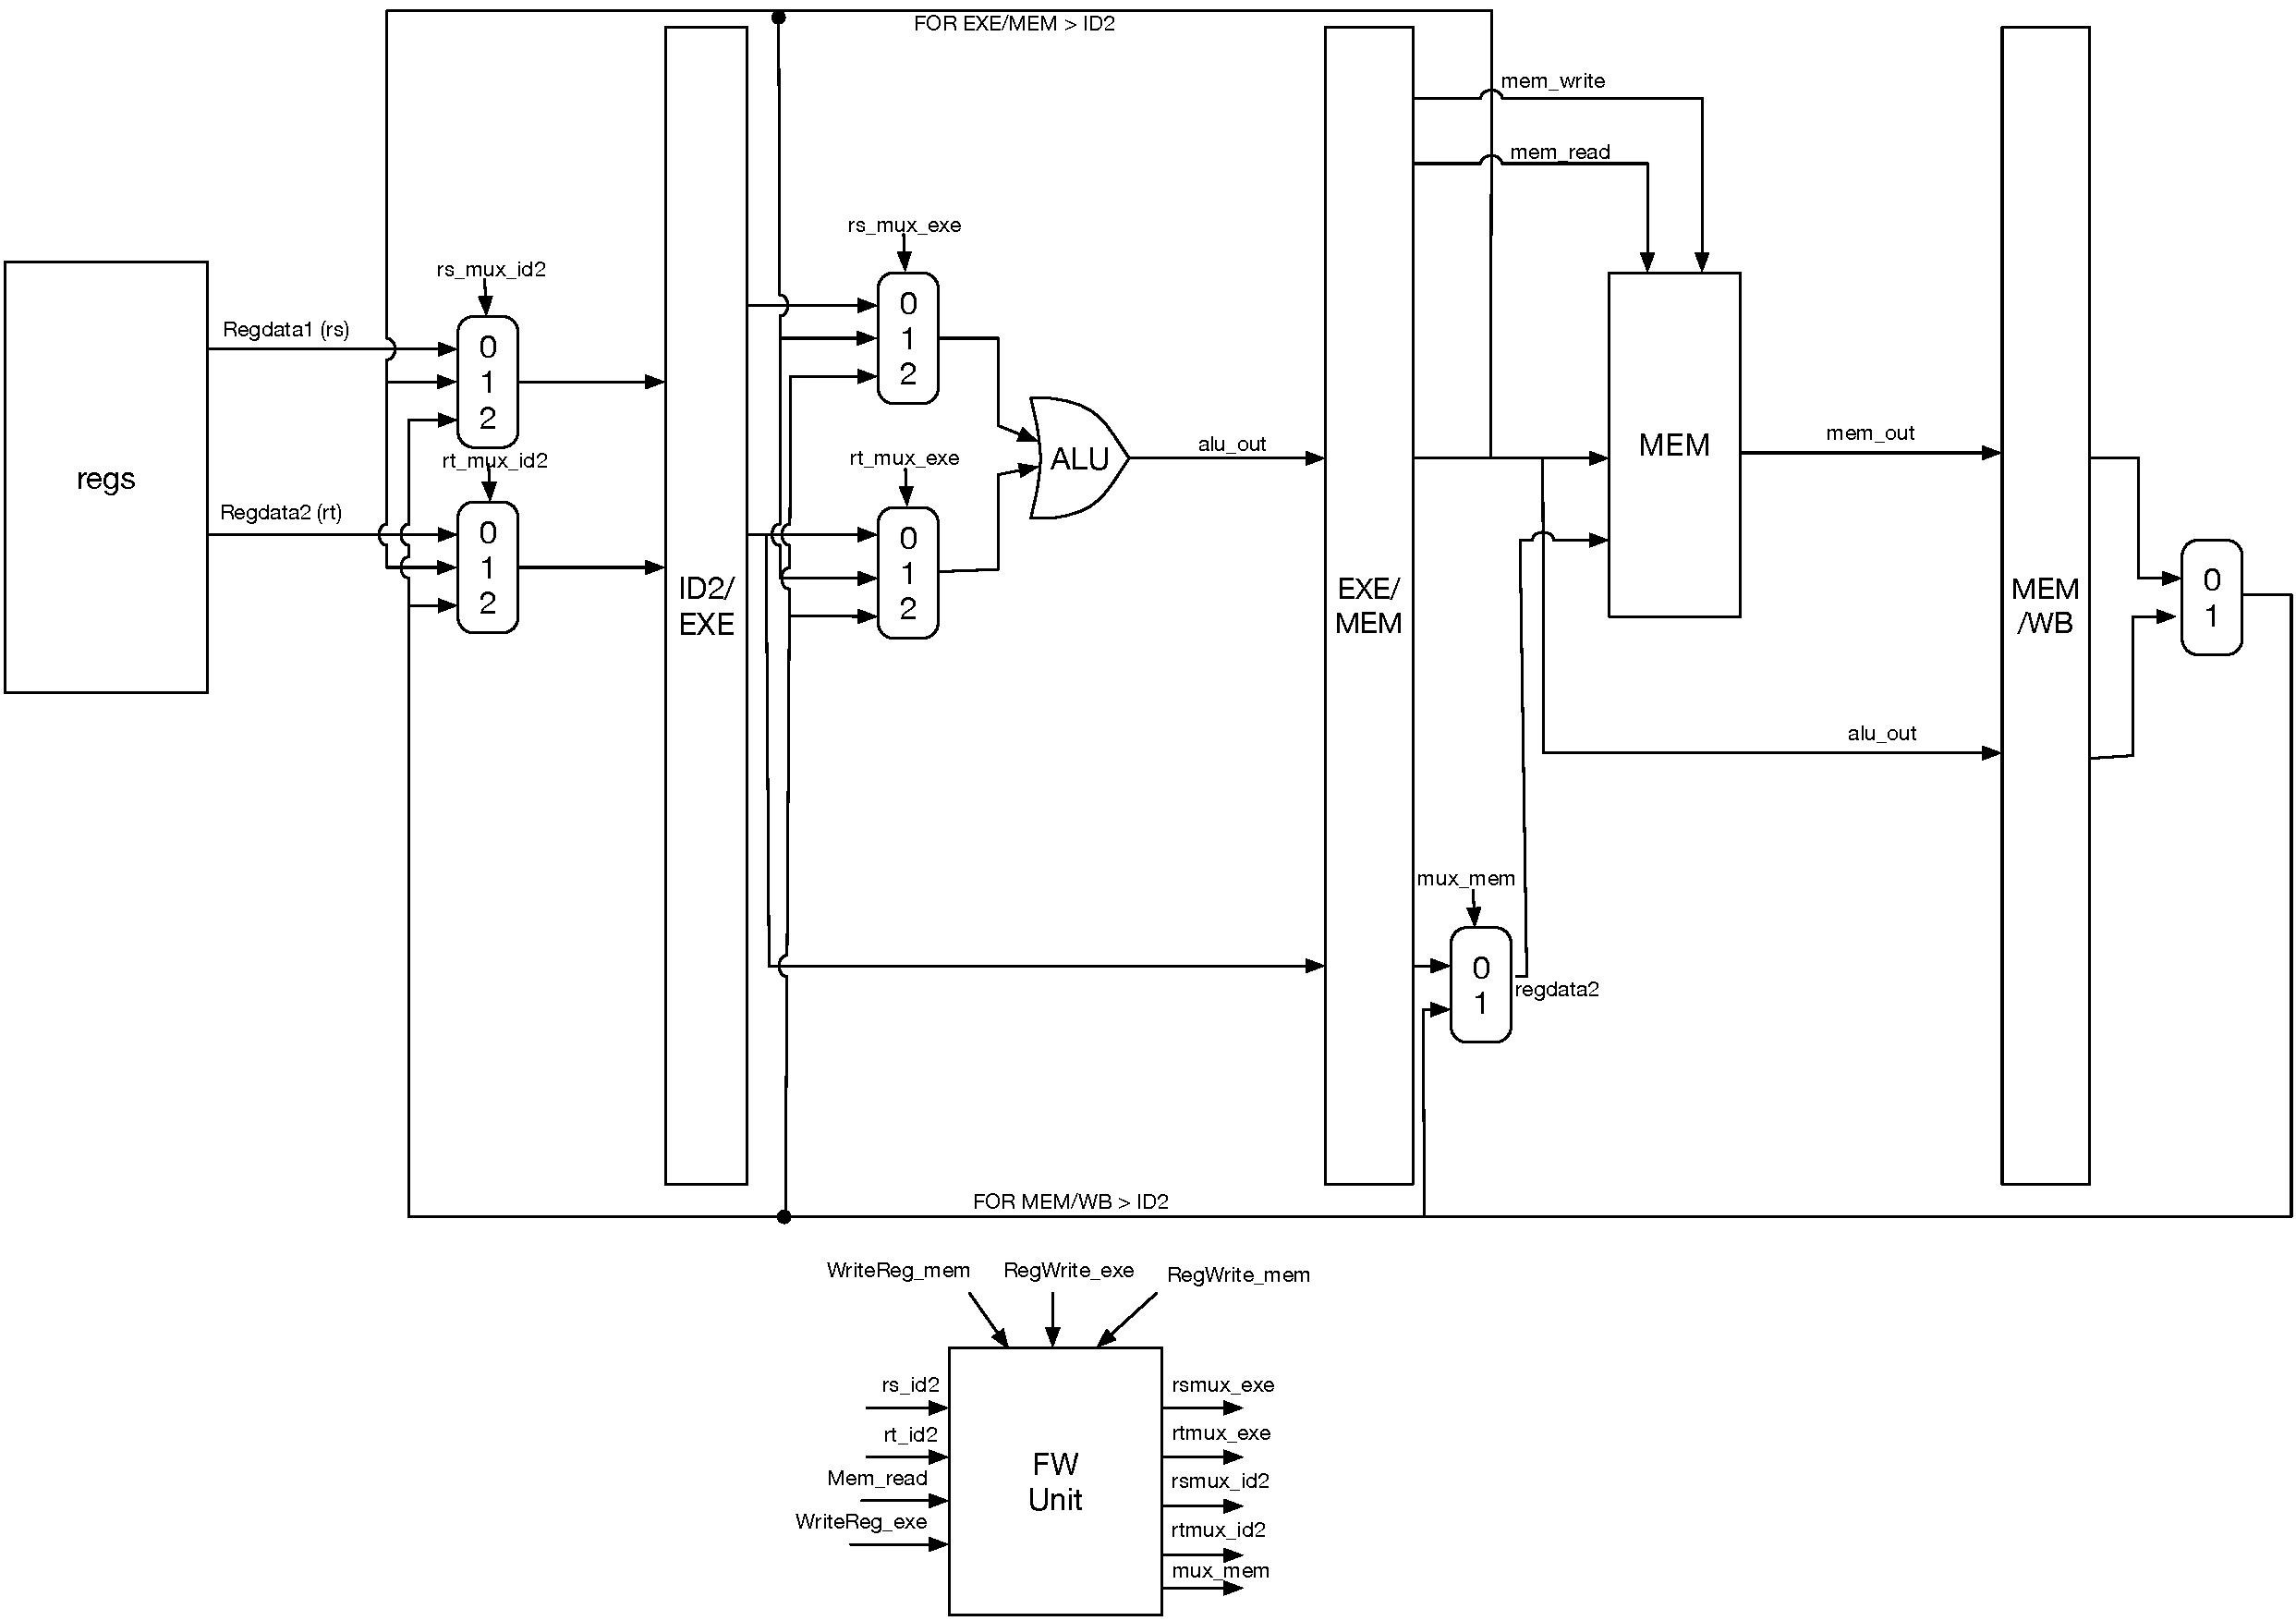
\includegraphics[width=150mm,scale=1]{path.pdf}
 \caption{\\ Forwarding path}
 \label{fig:path}
\end{figure}

\subsection{EXE/MEM->EXE}

\begin{table}[!htb]
\centering
\label{my-label}
\resizebox{\textwidth}{!}{\begin{tabular}{cc|c|c|
>{\columncolor[HTML]{F8A102}}c |
>{\columncolor[HTML]{FFCC67}}c |c|ccl}
\cline{2-7}
\multicolumn{1}{c|}{add \$1, \$2, \$3} & IF & ID1 & ID2 & EXE                                                & MEM                         & WB  &                         &  &  \\ \cline{2-8}
lw \$2, 0(\$1)                         &    & IF  & ID1 & \cellcolor[HTML]{FFFFFF}{\color[HTML]{000000} ID2} & \cellcolor[HTML]{F8A102}EXE & MEM & \multicolumn{1}{c|}{WB} &  &  \\ \cline{3-8}
\end{tabular}}
\end{table}

\begin{table}[!htb]
\centering
\label{for_ex_mem_exe}
\resizebox{\textwidth}{!}{\begin{tabular}{ll|c|c|l|
>{\columncolor[HTML]{FFCC67}}c |c|l}
\cline{2-7}
\multicolumn{1}{l|}{add \$1, \$2, \$3} & \multicolumn{1}{c|}{IF} & ID1 & ID2 & \multicolumn{1}{c|}{\cellcolor[HTML]{F8A102}EXE} & MEM                                                & WB  &                         \\ \cline{2-8} 
sub \$2, \$1, \$3                      &                         & IF  & ID1 & ID2                                              & \cellcolor[HTML]{F8A102}{\color[HTML]{333333} EXE} & MEM & \multicolumn{1}{c|}{WB} \\ \cline{3-8} 
\end{tabular}}
\end{table}

Este tipo de forwarding é causado por uma instrução que escreva num registo e de seguida uma outra instrução precise desse registo para realizar uma operação, ou seja, precisa de ler esse registo. Por exemplo, podemos ter um add \$1, \$2, \$3 e depois um sub \$2, \$1, \$3, a primeira instrução escreve em \$1 e a segunda instrução precisa do \$1  para realizar a operação de sub com \$3.
\linebreak

Tanto para RS e RT em ID2 comparamos com o WriteReg, se o registo RS/RT em ID2 é diferente de 0 e se vai escrever no registo ambos em EXE. 
Caso esta condição seja verdadeira, vamos então mudar o sinal de seleção do multiplexer para 1, sendo este sinal o que vai selecionar no mux o valor da entrada da ALU como "rs/rt".

Teve-se em atenção que o rt quando MemRead é verdadeiro é porque se vai escrever em rt, e o que nós queremos é ler em rt e não escrever em rt por isso adicionou-se a condição para que MemRead\_exe seja igual a false.
\linebreak

\begin{lstlisting}[language=c]
if(rs_exe.read()!=0 && rs_exe.read()==WriteReg_mem.read() 
	&& RegWrite_mem.read()==true){
    rs_mux_exe.write(1); 
}
if(rt_exe.read()!=0 && rt_exe.read()==WriteReg_mem.read() 
	&& RegWrite_mem.read()==true 
	&& MemRead_exe.read()==false){
   rt_mux_exe.write(1);
}
\end{lstlisting} 

\subsection{EXE/MEM->ID2}

\begin{table}[!htb]
\centering
\label{table_exe_mem_id2}
\resizebox{\textwidth}{!}{\begin{tabular}{ccc|c|c|c|c|cc}
\cline{2-7}
\multicolumn{1}{c|}{add \$1, \$2, \$3} & \multicolumn{1}{c|}{IF} & ID1 & ID2 & \cellcolor[HTML]{F8A102}EXE                        & \cellcolor[HTML]{FFCC67}MEM                        & WB  &                          &                         \\ \cline{2-8}
nop                                  & \multicolumn{1}{c|}{}   & IF  & ID1 & \cellcolor[HTML]{FFFFFF}{\color[HTML]{000000} ID2} & \cellcolor[HTML]{FFFFFF}{\color[HTML]{333333} EXE} & MEM & \multicolumn{1}{c|}{WB}  &                         \\ \cline{3-9} 
beq \$1, \$0, label                      &                         &     & IF  & ID1                                                & \cellcolor[HTML]{F8A102}{\color[HTML]{333333} ID2} & EXE & \multicolumn{1}{c|}{MEM} & \multicolumn{1}{c|}{WB} \\ \cline{4-9} 
\end{tabular}}
\end{table}

Este tipo de forwarding é causado por uma instrução que escreva num registo para o qual um branch condicional necessite de ler esse registo para tomar uma decisão. Por exemplo, neste caso, tem-se uma instrução add \$1, \$2, \$3 que vai escrever em \$1 e o beq vai necessitar de \$1 para calcular a decisão, neste caso é o \$rs mas também podia ser o \$rt o registo necessário para calcular a decisão que estivesse a ser escrito por uma outra instrução. É feito então o forwarding da fase EXE/MEM para ID2.

Nas condições que usamos para detetar estes casos de forwarding comparamos o rs/rt em id2 com o WriteReg em EXE, se vai escrever no registo em EXE e se é uma branch, ou seja, branch tem de ser diferente de 0, isto deve-se porque no exercício anterior colocou-se o sinal de branch a ter valores de 0 a 6. O multiplexer vai selecionar o forward de EXE/MEM para esta fase, fazendo com que os valores sejam selecionados os que está a ser feito o forward e não os que saem dos registos.

\begin{lstlisting}[language=c]
if(rs_id2.read()!=0 && rs_id2.read()==WriteReg_mem.read() 
	&& RegWrite_mem.read()==true && branch.read()!=0){
    rs_mux_id2.write(1);
}
if(rt_id2.read()!=0 && rt_id2.read()==WriteReg_mem.read() 
	&& RegWrite_mem.read()==true 
	&& branch.read()!=0 
	&& MemRead.read()==false){
   rt_mux_id2.write(1);
}
\end{lstlisting} 


\subsection{MEM/WB->EXE}

\begin{table}[!htb]
\centering
\label{my-label}
\resizebox{\textwidth}{!}{\begin{tabular}{ccc|c|c|c|c|cc}
\cline{2-7}
\multicolumn{1}{c|}{lw \$1, 0(\$0)} & \multicolumn{1}{c|}{IF} & ID1 & ID2 & EXE                                                & \cellcolor[HTML]{F8A102}MEM                        & \cellcolor[HTML]{FFCC67}WB  &                          &                         \\ \cline{2-8}
nop                               & \multicolumn{1}{c|}{}   & IF  & ID1 & \cellcolor[HTML]{FFFFFF}{\color[HTML]{000000} ID2} & \cellcolor[HTML]{FFFFFF}{\color[HTML]{333333} EXE} & MEM                         & \multicolumn{1}{c|}{WB}  &                         \\ \cline{3-9} 
add \$2, \$1, \$1                   &                         &     & IF  & ID1                                                & ID2                                                & \cellcolor[HTML]{F8A102}EXE & \multicolumn{1}{c|}{MEM} & \multicolumn{1}{c|}{WB} \\ \cline{4-9} 
\end{tabular}}
\end{table}

\begin{table}[!htb]
\centering
\label{my-label}
\resizebox{\textwidth}{!}{\begin{tabular}{ccc|c|c|c|c|cc}
\cline{2-7}
\multicolumn{1}{c|}{add \$1, \$0, \$0} & \multicolumn{1}{c|}{IF} & ID1 & ID2 & EXE                                                & \cellcolor[HTML]{F8A102}MEM                        & \cellcolor[HTML]{FFCC67}WB  &                          &                         \\ \cline{2-8}
nop                                  & \multicolumn{1}{c|}{}   & IF  & ID1 & \cellcolor[HTML]{FFFFFF}{\color[HTML]{000000} ID2} & \cellcolor[HTML]{FFFFFF}{\color[HTML]{333333} EXE} & MEM                         & \multicolumn{1}{c|}{WB}  &                         \\ \cline{3-9} 
add \$2, \$1, \$1                      &                         &     & IF  & ID1                                                & ID2                                                & \cellcolor[HTML]{F8A102}EXE & \multicolumn{1}{c|}{MEM} & \multicolumn{1}{c|}{WB} \\ \cline{4-9} 
\end{tabular}}
\end{table}

\begin{table}[!htb]
\centering
\resizebox{\textwidth}{!}{\begin{tabular}{ccc|c|c|c|c|cc}
\cline{2-7}
\multicolumn{1}{c|}{lw \$1, 0(\$0)} & \multicolumn{1}{c|}{IF} & ID1 & ID2 & EXE                                                & \cellcolor[HTML]{F8A102}MEM                        & \cellcolor[HTML]{FFCC67}WB  &                          &                         \\ \cline{2-8}
nop                               & \multicolumn{1}{c|}{}   & IF  & ID1 & \cellcolor[HTML]{FFFFFF}{\color[HTML]{000000} ID2} & \cellcolor[HTML]{FFFFFF}{\color[HTML]{333333} EXE} & MEM                         & \multicolumn{1}{c|}{WB}  &                         \\ \cline{3-9} 
lw \$1, 0(\$1)                      &                         &     & IF  & ID1                                                & ID2                                                & \cellcolor[HTML]{F8A102}EXE & \multicolumn{1}{c|}{MEM} & \multicolumn{1}{c|}{WB} \\ \cline{4-9} 
\end{tabular}}
\end{table}

Este tipo de forwarding é provocado por uma instrução do que escreva para um registo que uma terceira instrução na pipeline necessite de ler para efetuar a sua operação em EXE. 

Por exemplo, no nosso caso temos uma operação do tipo LW que lê na memória para o registo \$1, e depois, duas em EXE existe uma instrução que vai ler do registo que foi escrito pela instrução LW. Assim como podemos ter uma instrução do tipo R na fase MEM e uma instrução do tipo R que também necessite desse registo escrito pela primeira instrução na fase EXE. 

\begin{lstlisting}[language=c]
if(rs_exe.read()!=0 && rs_exe.read()==WriteReg_wb.read()
  && RegWrite_wb.read()==true){
    rs_mux_exe.write(2);
}
if(rt_exe.read()!=0 && rt_exe.read()==WriteReg_wb.read() 
  && RegWrite_wb.read()==true 
  && MemRead_exe.read()==false){
    rt_mux_exe.write(2);
}
\end{lstlisting} 

\subsection{MEM/WB->ID2}

\begin{table}[!htb]
\centering
\label{my-label}
\resizebox{\textwidth}{!}{\begin{tabular}{cccc|c|c|c|ccl}
\cline{2-7}
\multicolumn{1}{c|}{lw \$1, 0(\$0)}     & \multicolumn{1}{c|}{IF} & \multicolumn{1}{c|}{ID1} & ID2                   & EXE                                                & \cellcolor[HTML]{F8A102}MEM                        & \cellcolor[HTML]{FFCC67}WB  &                          &                          &                         \\ \cline{2-8}
nop                                   & \multicolumn{1}{c|}{}   & \multicolumn{1}{c|}{IF}  & ID1                   & \cellcolor[HTML]{FFFFFF}{\color[HTML]{000000} ID2} & \cellcolor[HTML]{FFFFFF}{\color[HTML]{333333} EXE} & MEM                         & \multicolumn{1}{c|}{WB}  &                          &                         \\ \cline{3-9}
nop                                   &                         & \multicolumn{1}{c|}{}    & IF                    & ID1                                                & ID2                                                & EXE                         & \multicolumn{1}{c|}{MEM} & \multicolumn{1}{c|}{WB}  &                         \\ \cline{4-10} 
\multicolumn{1}{l}{beq \$1, \$1, label} & \multicolumn{1}{l}{}    & \multicolumn{1}{l}{}     & \multicolumn{1}{l|}{} & IF                                                 & ID1                                                & \cellcolor[HTML]{F8A102}ID2 & \multicolumn{1}{c|}{EXE} & \multicolumn{1}{c|}{MEM} & \multicolumn{1}{c|}{WB} \\ \cline{5-10} 
\end{tabular}}
\end{table}

O caso de MEM/WB para ID2 apenas acontece quando existe uma instrução de leitura na memória e em que esse valor lido da memória apenas está disponível em WB e em ID2 está uma operação de beq ou outro tipo que leia um registo que está a para ser escrito pela instrução de lw. Será feito um forward desse valor de MEM/WB para ID2.

\begin{lstlisting}[language=c]
if(rs_id2.read()!=0 && rs_id2.read()==WriteReg_wb.read()
  && RegWrite_wb.read()==true){
    rs_mux_id2.write(2);
}
if(rt_id2.read()!=0 && rt_id2.read()==WriteReg_wb.read() 
  && RegWrite_wb.read()==true 
  && MemRead.read()==false){
    rt_mux_id2.write(2);
}
\end{lstlisting} 

\subsection{MEM/WB->MEM}
\begin{table}[!htb]
\centering
\label{my-label}
\resizebox{\textwidth}{!}{\begin{tabular}{cc|c|c|c|
>{\columncolor[HTML]{F8A102}}c |
>{\columncolor[HTML]{FFCC67}}c |ccl}
\cline{2-7}
\multicolumn{1}{c|}{lw \$1, 0(\$0)} & IF & ID1 & ID2 & EXE                                                & MEM                                                & WB                          &                         &  &  \\ \cline{2-8}
sw \$1, 0(\$0)                      &    & IF  & ID1 & \cellcolor[HTML]{FFFFFF}{\color[HTML]{000000} ID2} & \cellcolor[HTML]{FFFFFF}{\color[HTML]{333333} EXE} & \cellcolor[HTML]{F8A102}MEM & \multicolumn{1}{c|}{WB} &  &  \\ \cline{3-8}
\end{tabular}}
\end{table}

As condições para este caso acontecer são muito específicas, apenas dizem respeito a um lw seguido sw, não diz respeito a uma instrução do tipo R seguida de um sw porque nesse caso é feito o forward de EXE/MEM para EXE para resolver esse caso. Isto só acontece porque o lw só está disponível em MEM, ou seja, para a instrução de sw precisa na fase de MEM desse valor terá de ser feito o forward de MEM/WB para MEM. 
As condições são: em MemRead{\_}Wb==true, MemWrite{\_}Mem==true e WriteReg{\_}wb==rt{\_}mem!=0.

\begin{lstlisting}[language=c]
if(rt_mem.read()!=0 && rt_mem.read()==WriteReg_wb.read() 
  && RegWrite_wb.read()==true 
  && MemRead_wb.read()==true
  && MemWrite_mem.read()==true){
    mux_mem.write(1);
}
\end{lstlisting} 

\subsection{Forwarding para EXE}

\begin{table}[!htb]
\centering
\label{my-label}
\resizebox{\textwidth}{!}{\begin{tabular}{ccc|c|c|c|
>{\columncolor[HTML]{FFCB2F}}c |ccl}
\cline{2-7}
\multicolumn{1}{c|}{add \$1, \$2, \$3}                       & \multicolumn{1}{c|}{IF} & ID1                   & ID2 & EXE                                                & \cellcolor[HTML]{F8A102}MEM & WB                          &                          &                         &  \\ \cline{2-8}
add \$2, \$1, \$1                                            & \multicolumn{1}{c|}{}   & IF                    & ID1 & \cellcolor[HTML]{FFFFFF}{\color[HTML]{000000} ID2} & \cellcolor[HTML]{F8A102}EXE & MEM                         & \multicolumn{1}{c|}{WB}  &                         &  \\ \cline{3-9}
\multicolumn{1}{l}{{\color[HTML]{009901} add \$2, \$2, \$1}} & \multicolumn{1}{l}{}    & \multicolumn{1}{l|}{} & IF  & ID1                                                & ID2                         & \cellcolor[HTML]{F8A102}EXE & \multicolumn{1}{c|}{MEM} & \multicolumn{1}{c|}{WB} &  \\ \cline{4-9}
\end{tabular}}
\end{table}

Neste caso o forwarding é feito desde MEM/WB para EXE e de EXE/MEM para EXE. A instrução que está em EXE necessita dos valores que estão disponíveis na fase de MEM e WB que foram calculados em fases anteriores, sendo assim, é feito o forward para EXE desde MEM/WB e EXE/MEM. Também poderia ocorrer o caso de estar a ser calculado um endereço em EXE de uma instrução do tipo lw ou sw e então ser feito forward para esta fase de um valor que esteja a ser calculado numa das outras fases.

\subsection{Forwarding para ID2}

\begin{table}[!htb]
\centering
\label{my-label}
\resizebox{\textwidth}{!}{\begin{tabular}{lccc|c|c|c|ccc}
\cline{2-7}
\multicolumn{1}{l|}{lw \$1, 0(\$0)} & \multicolumn{1}{c|}{IF} & \multicolumn{1}{c|}{ID1} & ID2 & EXE & \cellcolor[HTML]{F8A102}MEM & \cellcolor[HTML]{FFCC67}WB  &                          &                          &                         \\ \cline{2-8}
add \$2,\$3, \$3                   & \multicolumn{1}{c|}{}   & \multicolumn{1}{c|}{IF}  & ID1 & ID2 & \cellcolor[HTML]{F8A102}EXE & \cellcolor[HTML]{FFCC67}MEM & \multicolumn{1}{c|}{WB}  &                          &                         \\ \cline{3-9}
nop                               &                         & \multicolumn{1}{c|}{}    & IF  & ID1 & ID2                         & EXE                         & \multicolumn{1}{c|}{MEM} & \multicolumn{1}{c|}{WB}  &                         \\ \cline{4-10} 
beq \$1, \$2, label                 &                         &                          &     & IF  & ID1                         & \cellcolor[HTML]{F8A102}ID2 & \multicolumn{1}{c|}{EXE} & \multicolumn{1}{c|}{MEM} & \multicolumn{1}{c|}{WB} \\ \cline{5-10} 
\end{tabular}}
\end{table}

\begin{table}[!htb]
\centering
\label{my-label}
\resizebox{\textwidth}{!}{\begin{tabular}{lccc|c|c|c|ccc}
\cline{2-7}
\multicolumn{1}{l|}{lw \$1, 0(\$0)} & \multicolumn{1}{c|}{IF} & \multicolumn{1}{c|}{ID1} & ID2 & EXE & \cellcolor[HTML]{F8A102}MEM & \cellcolor[HTML]{FFCC67}WB  &                          &                          &                         \\ \cline{2-8}
add \$2, \$3, \$3                   & \multicolumn{1}{c|}{}   & \multicolumn{1}{c|}{IF}  & ID1 & ID2 & EXE & MEM & \multicolumn{1}{c|}{WB}  &                          &                         \\ \cline{3-9}
nop                               &                         & \multicolumn{1}{c|}{}    & IF  & ID1 & ID2                         & EXE                         & \multicolumn{1}{c|}{MEM} & \multicolumn{1}{c|}{WB}  &                         \\ \cline{4-10} 
add \$2, \$1, \$2                   &                         &                          &     & IF  & ID1                         & \cellcolor[HTML]{F8A102}ID2 & \multicolumn{1}{c|}{EXE} & \multicolumn{1}{c|}{MEM} & \multicolumn{1}{c|}{WB} \\ \cline{5-10} 
\end{tabular}}
\end{table}

\begin{table}[!htb]
\centering
\label{my-label}
\resizebox{\textwidth}{!}{\begin{tabular}{lccc|c|c|c|ccc}
\cline{2-7}
\multicolumn{1}{l|}{lw \$1, 0(\$0)} & \multicolumn{1}{c|}{IF} & \multicolumn{1}{c|}{ID1} & ID2 & EXE & \cellcolor[HTML]{F8A102}MEM & \cellcolor[HTML]{FFCC67}WB  &                          &                          &                         \\ \cline{2-8}
nop                               & \multicolumn{1}{c|}{}   & \multicolumn{1}{c|}{IF}  & ID1 & ID2 & EXE                         & MEM                         & \multicolumn{1}{c|}{WB}  &                          &                         \\ \cline{3-9}
nop                               &                         & \multicolumn{1}{c|}{}    & IF  & ID1 & ID2                         & EXE                         & \multicolumn{1}{c|}{MEM} & \multicolumn{1}{c|}{WB}  &                         \\ \cline{4-10} 
lw \$2, 0(\$1)                      &                         &                          &     & IF  & ID1                         & \cellcolor[HTML]{F8A102}ID2 & \multicolumn{1}{c|}{EXE} & \multicolumn{1}{c|}{MEM} & \multicolumn{1}{c|}{WB} \\ \cline{5-10} 
\end{tabular}}
\end{table}

Neste caso assumimos que só está disponível o valor de \$1 quando o lw está na fase de MEM, e este é necessário por uma instrução que vai ler este registo. O valor só vai ser escrito no final de WB, e se o valor for necessário na fase ID2 então teremos de fazer forward. No caso do add, o resultado de um add, este só vai ser gravado quando terminar a fase de WB, no entanto pode ser feito o forward de EXE/MEM para ID2, pois este valor é necessário na fase ID2 (devido ao salto condicional). No caso do lw é necessário fazer o forward de MEM/WB para ID2, porque o valor também ainda não está disponível no banco de registo.

\subsection{Forwarding desde MEM/WB}

\begin{table}[!htb]
\centering
\label{my-label}
\resizebox{\textwidth}{!}{\begin{tabular}{lccc|c|c|
>{\columncolor[HTML]{F8A102}}c |ccc}
\cline{2-7}
\multicolumn{1}{l|}{lw \$1, 0(\$0)} & \multicolumn{1}{c|}{IF} & \multicolumn{1}{c|}{ID1} & ID2 & EXE & \cellcolor[HTML]{F8A102}MEM & \cellcolor[HTML]{FFCC67}WB &                          &                          &                         \\ \cline{2-8}
sw \$1, 8(\$0)                      & \multicolumn{1}{c|}{}   & \multicolumn{1}{c|}{IF}  & ID1 & ID2 & EXE                         & MEM                        & \multicolumn{1}{c|}{WB}  &                          &                         \\ \cline{3-9}
add \$2, \$1, \$1                   &                         & \multicolumn{1}{c|}{}    & IF  & ID1 & ID2                         & EXE                        & \multicolumn{1}{c|}{MEM} & \multicolumn{1}{c|}{WB}  &                         \\ \cline{4-10} 
lw \$2, 0(\$1)                      &                         &                          &     & IF  & ID1                         & ID2                        & \multicolumn{1}{c|}{EXE} & \multicolumn{1}{c|}{MEM} & \multicolumn{1}{c|}{WB} \\ \cline{5-10} 
\end{tabular}}
\end{table}

Este caso é quando existe um valor que tem de ser lido da memória, ou alguma operação do tipo R que foi calculado na fase de EXE  e é necessário para escrever na memória esse valor, entre a primeira e a segunda instrução existe uma dependência que tem de ser satisfeita através de um forward de MEM/WB para MEM. Outro caso é esse valor ser necessário para a operação que vai decorrer em EXE, fazendo assim um forward de MEM/WB para EXE. Outro caso é existir a necessidade de ler um registo que ainda não foi escrito e que a instrução que escreve nesse ainda não terminou, fazendo assim um forward de MEM/WB para ID2.


\subsection{Testes}

Foram pensados testes específicos para testar todos os forwards em conjunto, também é preciso salientar que todas os casos em cima foram testados individualmente.

\subsubsection{Teste 1}
Este teste pretende testar o forward de EXE/MEM para EXE e de MEM/WB para EXE.

\begin{table}[!htb]
\centering
\label{my-label}
\resizebox{\textwidth}{!}{\begin{tabular}{lcc|c|c|c|c|cc}
\cline{2-7}
\multicolumn{1}{l|}{add \$3, \$1, \$2} & \multicolumn{1}{c|}{IF} & ID1 & ID2 & \cellcolor[HTML]{F8A102}EXE & \cellcolor[HTML]{FFCC67}MEM & \cellcolor[HTML]{FFCC67}WB  &                          &                         \\ \cline{2-8}
add \$4, \$3, \$1                      & \multicolumn{1}{c|}{}   & IF  & ID1 & ID2                         & \cellcolor[HTML]{F8A102}EXE & MEM                         & \multicolumn{1}{c|}{WB}  &                         \\ \cline{3-9} 
add \$5, \$2, \$3                      &                         &     & IF  & ID1                         & ID2                         & \cellcolor[HTML]{F8A102}EXE & \multicolumn{1}{c|}{MEM} & \multicolumn{1}{c|}{WB} \\ \cline{4-9} 
\end{tabular}}
\end{table}

O segundo add vai necessitar de ler o \$3 que está a ser calculado  pelo primeiro add e está disponível nas fases MEM e WB. Sendo assim será feito forward de EXE/MEM para EXE para o segundo add e de MEM/WB para EXE por causa do terceiro add.

\subsubsection{Teste 2}

\begin{table}[!htb]
\centering
\label{my-label}
\resizebox{\textwidth}{!}{\begin{tabular}{lcccc|c|c|cccl}
\cline{2-7}
\multicolumn{1}{l|}{lw \$1, 0(\$0)} & \multicolumn{1}{c|}{IF} & \multicolumn{1}{c|}{ID1} & \multicolumn{1}{c|}{ID2} & EXE                   & MEM & WB                          &                                                  &                          &                          &                         \\ \cline{2-8}
lw \$2, 4(\$0)                      & \multicolumn{1}{c|}{}   & \multicolumn{1}{c|}{IF}  & \multicolumn{1}{c|}{ID1} & ID2                   & EXE & \cellcolor[HTML]{F8A102}MEM & \multicolumn{1}{c|}{\cellcolor[HTML]{FFCC67}WB}  &                          &                          &                         \\ \cline{3-9}
nop                               &                         & \multicolumn{1}{c|}{}    & \multicolumn{1}{c|}{IF}  & ID1                   & ID2 & EXE                         & \multicolumn{1}{c|}{MEM}                         & \multicolumn{1}{c|}{WB}  &                          &                         \\ \cline{4-10}
nop                               & \multicolumn{1}{l}{}    & \multicolumn{1}{l}{}     & \multicolumn{1}{l|}{}    & IF                    & ID1 & ID2                         & \multicolumn{1}{c|}{EXE}                         & \multicolumn{1}{c|}{MEM} & \multicolumn{1}{c|}{WB}  &                         \\ \cline{5-11} 
beq \$2, \$1, label                 & \multicolumn{1}{l}{}    & \multicolumn{1}{l}{}     & \multicolumn{1}{l}{}     & \multicolumn{1}{l|}{} & IF  & ID1                         & \multicolumn{1}{c|}{\cellcolor[HTML]{FFCC67}ID2} & \multicolumn{1}{c|}{EXE} & \multicolumn{1}{c|}{MEM} & \multicolumn{1}{c|}{WB} \\ \cline{6-11} 
\end{tabular}}
\end{table}

Este teste serve para testar um caso em que é necessário um valor no beq que está a ser calculado no segundo lw. Neste caso o forward é do tipo MEM/WB para ID2.

\newpage
\subsubsection{Teste 3}

\begin{table}[!htb]
\centering
\label{my-label}
\resizebox{\textwidth}{!}{\begin{tabular}{llllllllccclllllll}
\cline{2-7}
\multicolumn{1}{l|}{lw \$1, 0(\$0)} & \multicolumn{1}{c|}{IF} & \multicolumn{1}{c|}{ID1} & \multicolumn{1}{c|}{ID2} & \multicolumn{1}{c|}{EXE} & \multicolumn{1}{c|}{MEM} & \multicolumn{1}{c|}{WB}                          & \multicolumn{1}{c}{}                             &                                                  &                                                  & \multicolumn{1}{l}{}     &                          &                                                  &                                                  &                                                  &                          &                          &                         \\ \cline{2-8}
lw \$2, 4(\$0)                      & \multicolumn{1}{c|}{}   & \multicolumn{1}{c|}{IF}  & \multicolumn{1}{c|}{ID1} & \multicolumn{1}{c|}{ID2} & \multicolumn{1}{c|}{EXE} & \multicolumn{1}{c|}{\cellcolor[HTML]{F8A102}MEM} & \multicolumn{1}{c|}{\cellcolor[HTML]{FFCC67}WB}  &                                                  & \multicolumn{6}{l}{\textit{MEM/WB \textgreater EXE}}                                                                                                                                                                                                            &                          &                          &                         \\ \cline{3-9}
nop                               & \multicolumn{1}{c}{}    & \multicolumn{1}{c|}{}    & \multicolumn{1}{c|}{IF}  & \multicolumn{1}{c|}{ID1} & \multicolumn{1}{c|}{ID2} & \multicolumn{1}{c|}{EXE}                         & \multicolumn{1}{c|}{MEM}                         & \multicolumn{1}{c|}{WB}                          &                                                  & \multicolumn{1}{l}{}     &                          &                                                  &                                                  &                                                  &                          &                          &                         \\ \cline{4-10}
add \$3, \$2, \$1                   &                         &                          & \multicolumn{1}{l|}{}    & \multicolumn{1}{c|}{IF}  & \multicolumn{1}{c|}{ID1} & \multicolumn{1}{c|}{ID2}                         & \multicolumn{1}{c|}{\cellcolor[HTML]{FFCC67}EXE} & \multicolumn{1}{c|}{\cellcolor[HTML]{9AFF99}MEM} & \multicolumn{1}{c|}{\cellcolor[HTML]{FFFE65}WB}  & \multicolumn{1}{l}{}     & \multicolumn{7}{l}{\textit{EXE/MEM \textgreater EXE || MEM/WB \textgreater EXE || MEM/WB \textgreater ID2}}                                                                                                                                                       \\ \cline{5-11}
add \$4, \$3, \$1                   &                         &                          &                          & \multicolumn{1}{l|}{}    & \multicolumn{1}{c|}{IF}  & \multicolumn{1}{c|}{ID1}                         & \multicolumn{1}{c|}{ID2}                         & \multicolumn{1}{c|}{\cellcolor[HTML]{9AFF99}EXE} & \multicolumn{1}{c|}{\cellcolor[HTML]{FFFE65}MEM} & \multicolumn{1}{c|}{WB}  &                          &                                                  &                                                  &                                                  &                          &                          &                         \\ \cline{6-12}
add \$5, \$3, \$4                   &                         &                          &                          &                          & \multicolumn{1}{l|}{}    & \multicolumn{1}{l|}{IF}                          & \multicolumn{1}{l|}{ID1}                         & \multicolumn{1}{l|}{ID2}                         & \multicolumn{1}{l|}{\cellcolor[HTML]{FFFE65}EXE} & \multicolumn{1}{l|}{MEM} & \multicolumn{1}{l|}{WB}  &                                                  &                                                  &                                                  &                          &                          &                         \\ \cline{7-13}
add \$6, \$3, \$1                   &                         &                          &                          &                          &                          & \multicolumn{1}{l|}{}                            & \multicolumn{1}{l|}{IF}                          & \multicolumn{1}{l|}{ID1}                         & \multicolumn{1}{l|}{\cellcolor[HTML]{FCFF2F}ID2} & \multicolumn{1}{l|}{EXE} & \multicolumn{1}{l|}{MEM} & \multicolumn{1}{l|}{WB}                          &                                                  &                                                  &                          &                          &                         \\ \cline{8-14}
lw \$7, 0(\$0)                      &                         &                          &                          &                          &                          &                                                  & \multicolumn{1}{l|}{}                            & \multicolumn{1}{c|}{IF}                          & \multicolumn{1}{c|}{ID1}                         & \multicolumn{1}{c|}{ID2} & \multicolumn{1}{c|}{EXE} & \multicolumn{1}{c|}{\cellcolor[HTML]{F8A102}MEM} & \multicolumn{1}{c|}{\cellcolor[HTML]{FFCC67}WB}  &                                                  & \multicolumn{3}{l}{MEM/WB \textgreater MEM}                                   \\ \cline{9-15}
sw \$7, 4(\$0)                      &                         &                          &                          &                          &                          &                                                  &                                                  & \multicolumn{1}{l|}{}                            & \multicolumn{1}{c|}{IF}                          & \multicolumn{1}{c|}{ID1} & \multicolumn{1}{c|}{ID2} & \multicolumn{1}{c|}{EXE}                         & \multicolumn{1}{c|}{\cellcolor[HTML]{FFCC67}MEM} & \multicolumn{1}{c|}{WB}                          & \multicolumn{1}{c}{}     & \multicolumn{1}{c}{}     & \multicolumn{1}{c}{}    \\ \cline{10-16}
add \$8, \$1, \$2                   &                         &                          & \multicolumn{6}{r}{EXE/MEM \textgreater ID2}                                                                                                                                                                                            & \multicolumn{1}{c|}{}                            & \multicolumn{1}{c|}{IF}  & \multicolumn{1}{c|}{ID1} & \multicolumn{1}{c|}{ID2}                         & \multicolumn{1}{c|}{\cellcolor[HTML]{F8A102}EXE} & \multicolumn{1}{c|}{\cellcolor[HTML]{FFCC67}MEM} & \multicolumn{1}{c|}{WB}  & \multicolumn{1}{c}{}     & \multicolumn{1}{c}{}    \\ \cline{11-17}
nop                               &                         &                          &                          &                          &                          &                                                  &                                                  & \multicolumn{1}{l}{}                             &                                                  & \multicolumn{1}{c|}{}    & \multicolumn{1}{c|}{IF}  & \multicolumn{1}{c|}{ID1}                         & \multicolumn{1}{c|}{ID2}                         & \multicolumn{1}{c|}{EXE}                         & \multicolumn{1}{c|}{MEM} & \multicolumn{1}{c|}{WB}  & \multicolumn{1}{c}{}    \\ \cline{12-18} 
bne \$8, \$0, label                 &                         &                          &                          &                          &                          &                                                  &                                                  & \multicolumn{1}{l}{}                             &                                                  &                          & \multicolumn{1}{c|}{}    & \multicolumn{1}{c|}{IF}                          & \multicolumn{1}{c|}{ID1}                         & \multicolumn{1}{c|}{\cellcolor[HTML]{FFCC67}ID2} & \multicolumn{1}{c|}{EXE} & \multicolumn{1}{c|}{MEM} & \multicolumn{1}{c|}{WB} \\ \cline{13-18} 
\end{tabular}}
\end{table}

Neste teste pretendeu-se testar todos os tipos de forward, excluindo alguns que foram testados anteriormente. Os forwards presentes são: MEM/WB para EXE, EXE/MEM para EXE, MEM/WB para EXE, MEM/WB para ID2, MEM/WB para MEM e EXE/MEM para ID2.

\section{Forward e stalls}

No exercício 5, o último mas não menos importante, foi pedido que fosse identificado todas as condições que provocariam stall e posteriormente se mudasse a unidade de hazard para inserir stalls sempre que fosse identificado uma situação de stall.

\subsection{lw e lw}
\begin{table}[!htb]
\centering
\label{my-label}
\resizebox{\textwidth}{!}{\begin{tabular}{lc|c|c|c|c|
>{\columncolor[HTML]{FFCC67}}c |cccllll}
\cline{2-7}
\multicolumn{1}{l|}{lw \$1, 0(\$0)} & IF & ID1 & ID2 & EXE                         & \cellcolor[HTML]{F8A102}MEM & WB  &                          &                         &  &  &  &  &  \\ \cline{2-9}
lw \$2, 4(\$1)                      &    & IF  & ID1 & \cellcolor[HTML]{FFFE65}ID2 & ID2                         & EXE & \multicolumn{1}{c|}{MEM} & \multicolumn{1}{c|}{WB} &  &  &  &  &  \\ \cline{3-9}
\end{tabular}}
\end{table}

\begin{lstlisting}[language = c]
rs_id2.read()!=0 && rs_id2.read()==WriteReg_exe.read() 
&& RegWrite_exe.read()==true && MemRead_exe.read()==true
|| rt_id2.read()!=0 && rt_id2.read()==WriteReg_exe.read() 
&& RegWrite_exe.read()==true && MemRead_exe.read()==true 
&& MemRead.read()==false
\end{lstlisting}

Esta condição acontece porque o primeiro lw só tem o valor disponível em MEM/WB, após ter lido da memória, e como o segundo lw necessita desse valor em EXE para calcular o valor do endereço, então terá de ser feito um forward de MEM/WB para EXE. Para isso acontecer terá de ser feito um stall em ID2.

\newpage
\subsection{add e beq}
\begin{table}[!htb]
\centering
\label{my-label}
\resizebox{\textwidth}{!}{\begin{tabular}{lc|c|c|
>{\columncolor[HTML]{F8A102}}c |
>{\columncolor[HTML]{FFCC67}}c |c|cccllll}
\cline{2-7}
\multicolumn{1}{l|}{add \$1, \$0, \$0} & IF & ID1 & ID2 & EXE                         & MEM & WB  &                          &                         &  &  &  &  &  \\ \cline{2-9}
beq \$1, \$1, label                    &    & IF  & ID1 & \cellcolor[HTML]{FFFE65}ID2 & ID2 & EXE & \multicolumn{1}{c|}{MEM} & \multicolumn{1}{c|}{WB} &  &  &  &  &  \\ \cline{3-9}
\end{tabular}}
\end{table}


\begin{lstlisting}[language = c]
rs_id2.read()!=0 && rs_id2.read()==WriteReg_exe.read() 
&& RegWrite_exe.read()==true && branch.read()!=0
|| rt_id2.read()!=0 && rt_id2.read()==WriteReg_exe.read()
&& RegWrite_exe.read()==true && branch.read()!=0 
&& MemRead.read()==false
\end{lstlisting}

Este stall acontece quando um add tem um beq que necessite de ler o resultado do add. O resultado do add apenas está disponível em MEM (EXE/MEM) e WB(MEM/WB) para se ser feito o forward, mas, mesmo com o forward é preciso ser feito um stall em ID2 para o valor de EXE estar disponível e depois ser feito um forward de EXE/MEM para ID2 para que depois o beq conseguir calcular a condição de salto.

\subsection{lw e add}
\begin{table}[!htb]
\centering
\label{my-label}
\resizebox{\textwidth}{!}{\begin{tabular}{lc|c|c|c|c|
>{\columncolor[HTML]{FFCC67}}c |cccllll}
\cline{2-7}
\multicolumn{1}{l|}{lw \$1, 0(\$0)} & IF & ID1 & ID2 & EXE                         & \cellcolor[HTML]{F8A102}MEM & WB  &                          &                         &  &  &  &  &  \\ \cline{2-9}
add \$2, \$1, \$1                   &    & IF  & ID1 & \cellcolor[HTML]{FFFE65}ID2 & ID2                         & EXE & \multicolumn{1}{c|}{MEM} & \multicolumn{1}{c|}{WB} &  &  &  &  &  \\ \cline{3-9}
\end{tabular}}
\end{table}

\begin{lstlisting}[language = c]
rs_id2.read()!=0 && rs_id2.read()==WriteReg_exe.read() 
&& RegWrite_exe.read()==true && MemRead_exe.read()==true
|| rt_id2.read()!=0 && rt_id2.read()==WriteReg_exe.read() 
&& RegWrite_exe.read()==true && MemRead_exe.read()==true 
&& MemRead.read()==false
\end{lstlisting}

Neste caso tal como no primeiro caso, o valor lido da memória apenas está disponível na fase de WB, ou seja, é possível fazer forward de MEM/WB para outra fase. No nosso caso é feito forward diretamente para EXE causando um ciclo de stall. 
\newpage
\subsection{lw e beq}
\begin{table}[!htb]
\centering
\label{my-label}
\resizebox{\textwidth}{!}{\begin{tabular}{lc|c|c|c|
>{\columncolor[HTML]{F8A102}}c |
>{\columncolor[HTML]{FFCC67}}c |cccllll}
\cline{2-7}
\multicolumn{1}{l|}{lw \$1, 0(\$0)} & IF & ID1 & ID2 & EXE                         & MEM                         & WB  &                          &                          &                         &  &  &  &  \\ \cline{2-10}
beq \$1, \$1, label                 &    & IF  & ID1 & \cellcolor[HTML]{FFFE65}ID2 & \cellcolor[HTML]{FFFE65}ID2 & ID2 & \multicolumn{1}{c|}{EXE} & \multicolumn{1}{c|}{MEM} & \multicolumn{1}{c|}{WB} &  &  &  &  \\ \cline{3-10}
\end{tabular}}
\end{table}

\begin{lstlisting}[language = c]
rs_id2.read()!=0 && rs_id2.read()==WriteReg_exe.read() 
&& RegWrite_exe.read()==true && branch.read()!=0
|| rt_id2.read()!=0 && rt_id2.read()==WriteReg_exe.read()
&& RegWrite_exe.read()==true && branch.read()!=0 
&& MemRead.read()==false
|| rs_id2.read()!=0 && rs_id2.read()==WriteReg_mem.read() 
&& RegWrite_mem.read()==true && branch.read()!=0 
&& MemRead_mem.read()==true
|| rt_id2.read()!=0 && rt_id2.read()==WriteReg_mem.read() 
&& RegWrite_mem.read()==true && branch.read()!=0 
&& MemRead.read()==false && MemRead_mem.read()==true

\end{lstlisting}

Este é o único caso que provoca dois stalls em ID2. As condições de salto são calculadas em ID2 o que faz com que os valores que são usados para calcular a condição de salto têm de estar disponíveis em ID2 ou então é necessário que seja feito forward de barramentos da pipeline mais avançados para esta fase caso completem as necessidades. 

Neste caso o lw apenas tem disponível em MEM/WB o valor lido da memória para fazer forward para ID2 e assim a condição de salto pode ser calculada. Para que o lw leia da memória e depois faça o forward é necessário que o beq adicione dois stalls.

\newpage
\section{Conclusão}

Este trabalho foi útil para assentarmos todos os conhecimentos que fomos obtendo ao longo destes anos, tanto em Arquitectura de Computadores Avançada como em Arquitetura de Computadores I e II. Ambas as entregas foram primeiro planeadas em papel antes de se avançar para a implementação o que resultou em bons resultados a nível de tempo despendido, para ambos as entregas fez-se uso de dois dias de trabalho.

Na primeira entrega houve uma falha na implementação, esqueceu-se de realizar o shift left 2 do program counter para calcular o endereço para onde é suposto saltar a instrução jump.

Já na segunda entrega teve-se os máximos cuidados para que tudo funcionasse perfeitamente.

\end{document}